%!TEX program = xelatex 
\documentclass{standalone}%opcao draft remove os links
\usepackage{amssymb,amsmath,amsfonts,amsthm,amstext,pxfonts}
\usepackage{graphicx}
\usepackage[usenames,dvipsnames]{xcolor}
\usepackage{subfigure}
\usepackage{tikz,tikz-3dplot,tkz-euclide,circuitikz,siunitx,pstricks-add,pst-coil,pst-3dplot}
\usepackage{pst-plot,pst-func,pst-eucl,pst-solides3d}
\usetkzobj{all}
\usetikzlibrary{scopes}
\usetikzlibrary{through}
\usetikzlibrary{lindenmayersystems}
\usetikzlibrary[shadings]
\usetikzlibrary{arrows}
\usetikzlibrary{intersections,positioning}

\newcommand{\norm}[1]{\left\Vert{#1}\right\Vert}
\newcommand{\eq}{=}

\begin{document}
    \pagenumbering{gobble}
    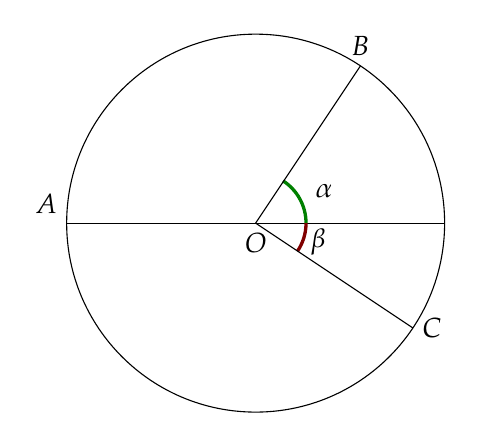
\begin{tikzpicture}[scale=.8]
      \coordinate [label=-90:$O$](o) at (3,0);
      \coordinate [label=150:$A$](a) at (0,0);
      \coordinate (b) at (6,0);%ponto B
      \coordinate (c) at (5,3);%ponto C
      \coordinate (d) at (6,-2);%ponto D
      \draw (a) -- (b);
      \node(c1) at (o)[draw,circle through=(a)] {};
      \coordinate [label=$B$](e) at (intersection 1 of c1 and o--c);
      \coordinate [label=0:$C$](f) at (intersection 1 of c1 and o--d);
      \coordinate (g) at (4,-0.3);
      \draw [green!50!black,very thick](o) +(0:.8cm) arc (0:57:.8cm);
      \draw [color=black](o)+(25:1.2) node[rotate=0] {$\alpha$};
      \draw [red!50!black,very thick](o) +(0:.8cm) arc (0:-34:.8cm);
      \draw [color=black](g) node[rotate=0] {$\beta$};
      \draw (o) -- (e);
      \draw (o) -- (f);
    \end{tikzpicture}
\end{document}